\chapter{Modelo proposto}\label{cap:proposta}
Neste capítulo se discutirá a proposta do sistema e seu desenvolvimento, será exposto como funciona todo o ambiente simulado. Dentre os sistemas que compõe um veículo autônomo o foco deste projeto será em desenvolver o componente de controle de deslocamento, isto é, ao agente é dado um trajeto o qual deve percorrer. O trajeto, em um contexto real seria definido por outro componente, porém aqui é predefinido pelo autor, não há necessidade de que os percursos sejam o mais eficiente possível, em vez disso o conjunto destes devem oferecer uma variedade de manobras a serem feitas pelo agente.

% Esta seção está sujeita a mudanças feitas no ambiente durante o PGCIII. 

\section{Ambiente}
A simulação envolve em treinar o veículo para percorrer trajetos em ambiente urbano, a princípio, por uma questão de simplicidade o agente não terá de lidar com declives ou aclives, semáforos, outros veículos ou pedestres. Porém outros elementos estáticos comuns de uma cidade como calçadas, postes, árvores, prédios, etc. Portanto, o foco poderá se manter no estudo de fazer um agente percorrer as rotas. Às bordas do cenário há muros que limitam o alcance do veículo, foi concluído pelo autor que o tamanho atual é suficiente para os treinos iniciais, em estudos futuros pode ser considerado a expansão do cenário.

\begin{figure}[h]
   \centering
   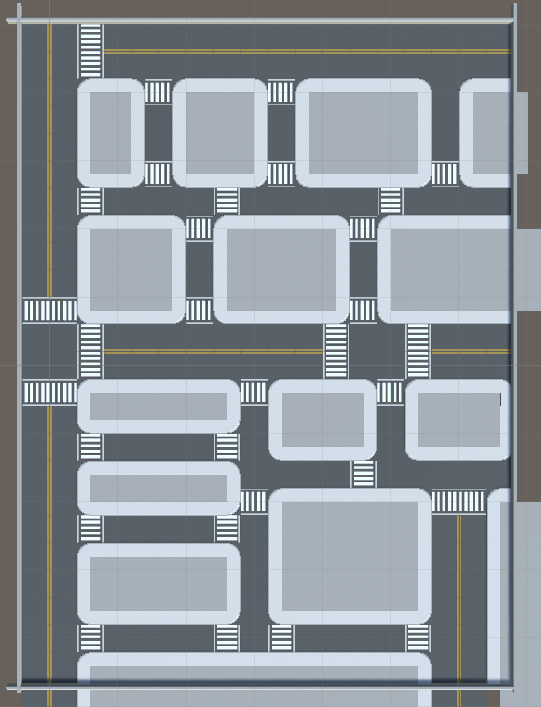
\includegraphics[scale=0.5, angle=90]{figs/Mapa-simulador-visao-superior.png}
    \caption{Visão superior o cenário urbano criado para o treinamento do veículo}
    \label{fig:map-view}
 \end{figure}

As rotas são compostas por: origem, \textit{checkpoints} e destino. O primeiro indica o local de partida do veículo, o último é o objetivo final do agente naquele episódio. Os \textit{checkpoints} são barreiras que indicam o caminho que deve ser percorrido, cada vez que o veículo atravessa uma delas ele ganha uma recompensa, isto é uma forma de indicar a ele que está fazendo o correto. Há 16 percursos predefinidos, cada uma delas possuem características distintas como distância origem-destino, quais e quantas conversões a serem feitas, isto fora pensado visando trazer uma diversidade maior de desafios a serem superados pelo agente. Assim como o tamanho do cenário, novos trajetos podem ser considerados em estudos futuros.

\begin{figure}[h]
   \centering
   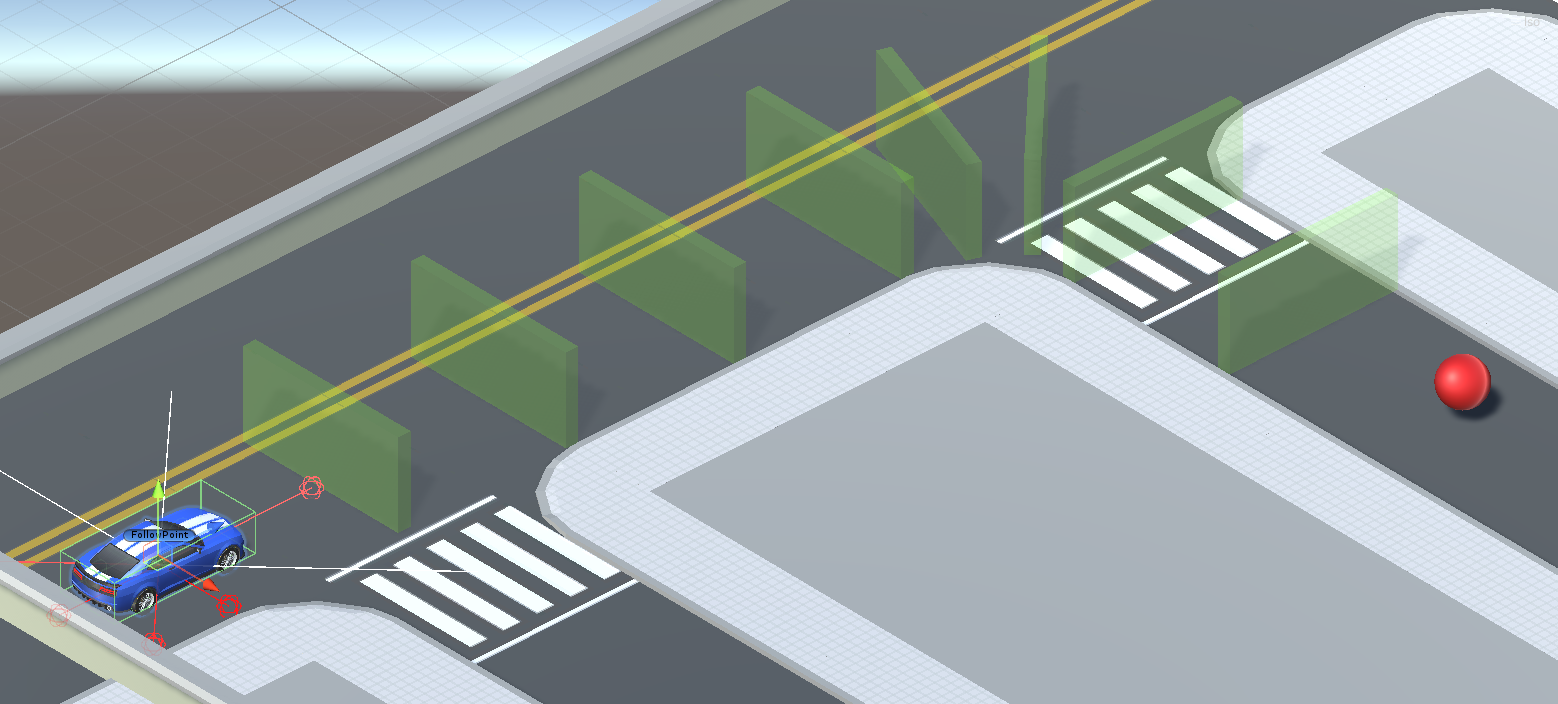
\includegraphics[scale=0.35]{figs/detalhe-rota.png}
    \caption{Rota vista de perspectiva isométrica, o agente posicionado a origem ao canto esquerdo, com os \textit{checkpoints} ao longo do percurso até o destino no canto direito.}
    \label{fig:route-view}
 \end{figure}

 \section{Agente}
 Para o aprendizado o veículo possui 8 sensores apontando para todas as direções uniformemente espaçadas, estes sensores são um \textit{component} do pacote \textbf{ML-agents} da Unity3D, são capazes de medir a distância dos objetos próximos ao veículo e também são capazes de distinguir quais são estes objetos. Estes sensores dentro do editor são representado por raio que partem do centro do veículo é possível configurar a diversos atributos deles como a quantidade, o ângulo máximo de distância do primeiro ao último, o ângulo vertical (que indica se eles apontam para cima ou para baixo) e o tamanho da esfera, que nada mais é que a tolerância de colisão do sensor.

 Além dos sensores, foi adicionado a velocidade do veículo a lista de observações do agente. Vale lembrar que o não foi implementado um recurso de imagem em um primeiro momento, ou seja, o veículo só enxerga através dos sensores e tem ciência de sua própria velocidade, ele é "cego" a qualquer outro elemento do ambiente que não esteja se choccando com o sensor.

 \begin{figure}[h]
   \centering
   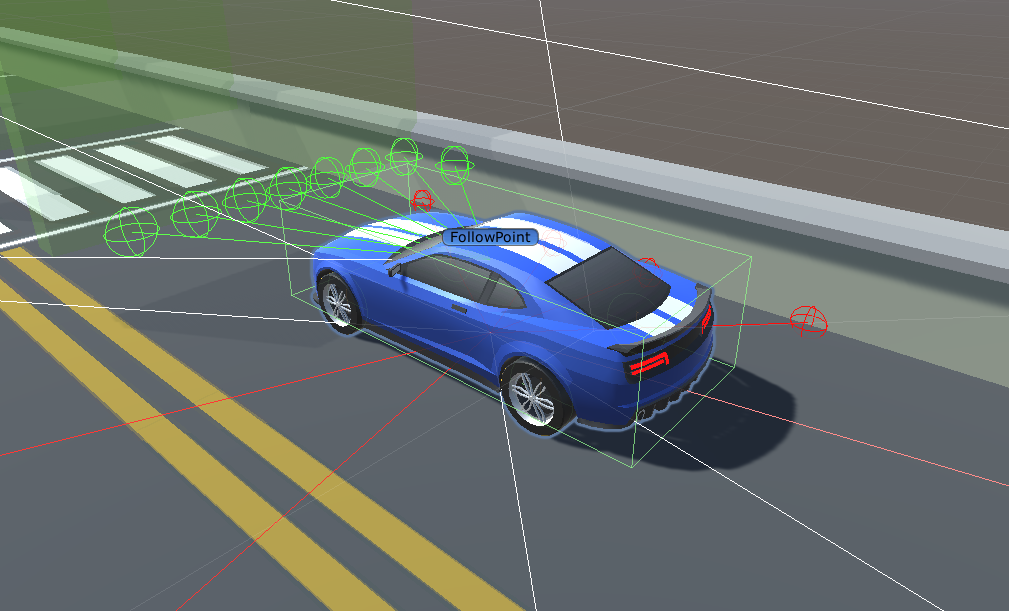
\includegraphics[scale=0.35]{figs/agente-raios-checkpoint.png}
    \caption{Exemplo do agente e seus raios perceptores, é possível ver 6 raios laterais se chocando com as calçadas ao lado, o raio frontal se chocando com o \textit{checkpoint}.}
    \label{fig:casting-rays}
 \end{figure}

 Quanto as ações que o agente pode fazer são apenas 3: acelerar, frear e direcionar as rodas a direita e a esquerda. A primeira e a última ação são chamadas ações contínuas, sendo assim um número que indica o nível de aceleração que o carro irá produzir, e no caso da direção da roda o quão direciona elas estão a esquerda ou direita. O ato de frear por outro lado é uma grandeza discreta e binária, não há pouca ou muita frenagem, simplesmente o veículo está ou não está freando.

 \section{Roteiro de treino}
 